%%%%%%%%%%%%%%%%%%%%%%%%%%%%%%%%%%%%%%%%%
% Proceedings of the National Academy of Sciences (PNAS)
% LaTeX Template
% Version 1.0 (19/5/13)
%
% This template has been downloaded from:
% http://www.LaTeXTemplates.com
%
% Original author:
% The PNAStwo class was created and is owned by PNAS:
% http://www.pnas.org/site/authors/LaTex.xhtml
% This template has been modified from the blank PNAS template to include
% examples of how to insert content and drastically change commenting. The
% structural integrity is maintained as in the original blank template.
%
% Original header:
%% PNAStmpl.tex
%% Template file to use for PNAS articles prepared in LaTeX
%% Version: Apr 14, 2008
%
%%%%%%%%%%%%%%%%%%%%%%%%%%%%%%%%%%%%%%%%%

%----------------------------------------------------------------------------------------
%	PACKAGES AND OTHER DOCUMENT CONFIGURATIONS
%----------------------------------------------------------------------------------------

%------------------------------------------------
% BASIC CLASS FILE
%------------------------------------------------

%% PNAStwo for two column articles is called by default.
%% Uncomment PNASone for single column articles. One column class
%% and style files are available upon request from pnas@nas.edu.

%\documentclass{pnasone}
\documentclass{pnastwo}

%------------------------------------------------
% POSITION OF TEXT
%------------------------------------------------

%% Changing position of text on physical page:
%% Since not all printers position
%% the printed page in the same place on the physical page,
%% you can change the position yourself here, if you need to:

% \advance\voffset -.5in % Minus dimension will raise the printed page on the 
                         %  physical page; positive dimension will lower it.

%% You may set the dimension to the size that you need.

%------------------------------------------------
% GRAPHICS STYLE FILE
%------------------------------------------------

%% Requires graphics style file (graphicx.sty), used for inserting
%% .eps/image files into LaTeX articles.
%% Note that inclusion of .eps files is for your reference only;
%% when submitting to PNAS please submit figures separately.

%% Type into the square brackets the name of the driver program 
%% that you are using. If you don't know, try dvips, which is the
%% most common PC driver, or textures for the Mac. These are the options:

% [dvips], [xdvi], [dvipdf], [dvipdfm], [dvipdfmx], [pdftex], [dvipsone],
% [dviwindo], [emtex], [dviwin], [pctexps], [pctexwin], [pctexhp], [pctex32],
% [truetex], [tcidvi], [vtex], [oztex], [textures], [xetex]

\usepackage{graphicx}

%------------------------------------------------
% OPTIONAL POSTSCRIPT FONT FILES
%------------------------------------------------

%% PostScript font files: You may need to edit the PNASoneF.sty
%% or PNAStwoF.sty file to make the font names match those on your system. 
%% Alternatively, you can leave the font style file commands commented out
%% and typeset your article using the default Computer Modern 
%% fonts (recommended). If accepted, your article will be typeset
%% at PNAS using PostScript fonts.

% Choose PNASoneF for one column; PNAStwoF for two column:
%\usepackage{PNASoneF}
%\usepackage{PNAStwoF}

%------------------------------------------------
% ADDITIONAL OPTIONAL STYLE FILES
%------------------------------------------------

%% The AMS math files are commonly used to gain access to useful features
%% like extended math fonts and math commands.

\usepackage{amssymb,amsfonts,amsmath}

%------------------------------------------------
% OPTIONAL MACRO FILES
%------------------------------------------------

%% Insert self-defined macros here.
%% \newcommand definitions are recommended; \def definitions are supported

%\newcommand{\mfrac}[2]{\frac{\displaystyle #1}{\displaystyle #2}}
%\def\s{\sigma}

%------------------------------------------------
% DO NOT EDIT THIS SECTION
%------------------------------------------------

%% For PNAS Only:
\contributor{Submitted to Proceedings of the National Academy of Sciences of the United States of America}
\url{www.pnas.org/cgi/doi/10.1073/pnas.0709640104}
\copyrightyear{2008}
\issuedate{Issue Date}
\volume{Volume}
\issuenumber{Issue Number}

%----------------------------------------------------------------------------------------

\begin{document}

%----------------------------------------------------------------------------------------
%	TITLE AND AUTHORS
%----------------------------------------------------------------------------------------

\title{Dimensionality Reduction in Modeling Transcriptome Dynamics} % For titles, only capitalize the first letter

%------------------------------------------------

%% Enter authors via the \author command.  
%% Use \affil to define affiliations.
%% (Leave no spaces between author name and \affil command)

%% Note that the \thanks{} command has been disabled in favor of
%% a generic, reserved space for PNAS publication footnotes.

%% \author{<author name>
%% \affil{<number>}{<Institution>}} One number for each institution.
%% The same number should be used for authors that
%% are affiliated with the same institution, after the first time
%% only the number is needed, ie, \affil{number}{text}, \affil{number}{}
%% Then, before last author ...
%% \and
%% \author{<author name>
%% \affil{<number>}{}}

%% For example, assuming Garcia and Sonnery are both affiliated with
%% Universidad de Murcia:
%% \author{Roberta Graff\affil{1}{University of Cambridge, Cambridge,
%% United Kingdom},
%% Javier de Ruiz Garcia\affil{2}{Universidad de Murcia, Bioquimica y Biologia
%% Molecular, Murcia, Spain}, \and Franklin Sonnery\affil{2}{}}

\author{Thomas Wood\affil{1}{Wood Gesellschaft Applied Physics Laboratory},  
Eli Shlizerman\affil{2}{University of Washington}}

\contributor{Submitted to Proceedings of the National Academy of Sciences
of the United States of America}

%----------------------------------------------------------------------------------------

\maketitle % The \maketitle command is necessary to build the title page

\begin{article}

%----------------------------------------------------------------------------------------
%	ABSTRACT, KEYWORDS AND ABBREVIATIONS
%----------------------------------------------------------------------------------------

\begin{abstract}
The number of genes in the genome of even a simple organism such as the Baker's yeast make modeling genome expression dynamics a non-trivial problem in Systems Biology. Dimensionality Reduction through Singular Value Decomposition (SVD) can help reduce the number of relevant features of genome expression and therefore aid in the fitting of macroscale dynamical models to genomic expression data. Due to the linear nature of the SVD, it is possible to extrapolate a microscale model by using a macroscale model of the genome expression dynamics to infer functional relationships between genes using time-series microarray data alone. We use our method to seek information about which genes in S. cerevisiae are affected by a combination therapy of Phenelzine and Lithium which is known to affect genome-level patterns of gene expression.
\end{abstract}

%------------------------------------------------

\keywords{Transcriptome Dynamics | Nonlinear Optimization | Singular Value Decomposition} % When adding keywords, separate each term with a straight line: |

%------------------------------------------------

%% Optional for entering abbreviations, separate the abbreviation from
%% its definition with a comma, separate each pair with a semicolon:
%% for example:
%% \abbreviations{SAM, self-assembled monolayer; OTS,
%% octadecyltrichlorosilane}

% \abbreviations{}
\abbreviations{SVD, Singular Value Decomposition; IDK, I Don't Know}

%----------------------------------------------------------------------------------------
%	PUBLICATION CONTENT
%----------------------------------------------------------------------------------------

%% The first letter of the article should be drop cap: \dropcap{} e.g.,
%\dropcap{I}n this article we study the evolution of ''almost-sharp'' fronts

\section{Introduction}

\dropcap{T}he large number of genes in the genome of the Baker's yeast make modeling the dynamics of the expression of the genome a difficult task to undertake\cite{10}. Due to the high number of dimensions in the problem of finding a dynamical model to fit to genome expression data, even finding a linear relationship between genes in the form of a transition matrix becomes untenably difficult. Predicting the expression levels of all the genes in the genome of S. cerevisiae through the use of a transition matrix with roughly 25 million parameters can be accomplished through projecting the time series genome expression data into a space where the genes are clustered into orthogonal components that correspond to the frequency with which changes in the expression of the clusters occur.


We used genome expression data of the form
\begin{equation}
X = \begin{bmatrix}
  \vec{x}_1 & \vec{x}_2 & \cdots & \vec{x}_N
\end{bmatrix}, \label{eq1}
\end{equation}
%\eqref{eq1}
where $\vec{x_i}$ refers to the gene expression for $M = 5619$ of the genes of S. cerevisiae which we were able to map from the Affymetrix Yeast 2.0 microarray identifiers to ENSEMBL gene ids for the $i$-th time series measurement.
%Referencing equation \eqref{qg1}. 

Through applying the SVD, we were able to decompose our matrix $X$ into the product of three matrices $U, \Sigma, $ and $ V^{*}$
\begin{equation}
X = U \Sigma V^{*} \label{eq2} \end{equation} ,which we can also write as
\begin{equation}
\begin{bmatrix}\vec{x}_1 & \cdots & \vec{x}_N\end{bmatrix}
= \begin{bmatrix} \vec{u}_1 & \cdots & \vec{u}_M \end{bmatrix}
\begin{bmatrix} \sigma_1 &  & \\
 & \ddots & \\
& & \sigma_N \\
0 & 0 & 0 \\
\vdots & \vdots & \vdots 
\end{bmatrix}
\begin{bmatrix} \vec{v}^1 \\
\vdots \\
\vec{v}^N
\end{bmatrix},\label{eq3}
\end{equation}
where $\vec{u}_i$ is a $rank(M)$ basis column-vector which represents the topology of the $i$-th mode of the genome expression time series matrix and $U$ is a M X M orthogonal matrix, $\Sigma$ is a M X N matrix of singular values of the first N modes, and the N X N matrix $V^{*}$ is composed of row-vectors $\vec{v}^i$ that represent the dynamics of the $i$-th mode in the original time-series matrix $X$.

From \eqref{eq3}, we can determine that 
\begin{equation}\vec{x_t} = \sum_k \vec{u}_k \sigma_k v_{t}^k,\label{eq4}
\end{equation}
where $v_{t}^k$ represents the value of the $k$-th mode at time $t$. Taking the inner product of both sides of \eqref{eq4} with $\vec{u}_j$ and using the fact that $\langle \vec{u}_k, \vec{u}_j \rangle =1$ if $j=k$ and $0$ otherwise, we find
\begin{align}
\langle \vec{u}_j, \vec{x}_t \rangle &= \langle \vec{u}_j, \sum_k \vec{u}_k \sigma_k v_{k}^t \rangle \\ &= \sigma_j v_{t}^j \text{   thus, }\\
v_{t}^j &= \langle \vec{u}_j, \vec{x}_t \rangle / \sigma_j.\label{eq7}\end{align}

To model the expression of the genome modes, we sought an optimal transition matrix $T$ by using nonlinear conjugate gradient descent to minimize an $L2$ error function, thereby arriving at a difference equation
\begin{align}
\vec{v}_{t+1} &= T \vec{v}_t \text{ or, }\\
v_{t+1}^{i} &= \sum_j T_{j}^i v_{t}^j,\label{eq9}
\end{align}
where $\vec{v}_t$ represents a column vector of the expression of each mode being considered at time $t$. Because each dimension of the difference equation represents a single genome mode, the oscillations which arise from our difference equation are solely the result of couplings between the first-order systems which model each genome mode.

In order to find a microscale model for the genome expression dynamics, we needed to find a formula relating $x_{t+1}^{r}$, the expression of the $r$-th gene at time $t+1$, to $\vec{x}_t$. This will allow us to find an M X M transition matrix $W$ that can step forward in time the expression levels of the entire genome
\begin{equation}
\vec{x}_{t+1} = W \vec{x}_t. \label{eq10}
\end{equation}

From considering only the $r$-th entry of the vector equation \eqref{eq4}, we can write
\begin{equation}
x_{t+1}^r = \sum_i u_{i}^r \sigma_i v_{t+1}^{i}.\label{eq11}
\end{equation}

Plugging \eqref{eq9} into \eqref{eq11}, we can see
\begin{equation}
x_{t+1}^r = \sum_i u_i^r \sigma_i ( \sum_j T_j^i v_{t}^j )
\label{eq12}
\end{equation}
and by further substituting \eqref{eq7} into \eqref{eq12} we arrive
at the expression
\begin{equation}
x_{t+1}^r = \sum_i u_i^r \sigma_i ( \sum_j T_j^i \langle \vec{u}_j, \vec{x}_t \rangle / \sigma_j. )
\label{eq13}
\end{equation}

On examining \eqref{eq13} we can see that $\vec{x}_t$ is the same for all $i$ and $j$, thus it is now apparent that we may write the $r$-th row vector of the microscale transition matrix W from \eqref{eq10} as

\begin{equation}
\vec{w}^r = \sum_i u_i^r \sigma_i ( \sum_j T_i^j \vec{u}_j / \sigma_j ). \qquad \qquad \Box
\label{eq14}
\end{equation}

%------------------------------------------------

\section{Results}

Referencing Table \ref{sampletable}. Referencing Figure \ref{Figure2}.

\subsection{Simulations}

\subsubsection{Simulation 1}

I don't know why they wrote in Latin all of the text in the template.

\subsubsection{Simulation 2}

I am not sure if we are going to have a section named {\em Simulation}.

\subsection{Real Data}

The layout of the template is confusing.

%------------------------------------------------

\section{Discussion}

This is the section where we can give a good discussion about how the different methods of parameter estimation to fit the ODE to the genome modes worked (and didn't work) as well as plausible reasons why.

%----------------------------------------------------------------------------------------
%	MATERIALS AND METHODS
%----------------------------------------------------------------------------------------

%% Optional Materials and Methods Section
%% The Materials and Methods section header will be added automatically.

\begin{materials}
This section will contain a description of the software modules we used to.

\begin{definition}
I'm going to leave this part alone for right now. A bounded function
$\theta$ is a weak solution of QG if for any 
$\phi\,\epsilon\, C_0^{\infty}(\fdb\times\mathbb{R}\times[0,\vep])$ we have
\begin{eqnarray}
&&  \int_{\mathbb{R}^+\times\fd\times\mathbb{R}} \hspace{-25pt}
 \theta(x,y,t)\, \pr_t \phi
\,(x,y,t) dy dx dt+\nonumber\\
  & +&\int_{\mathbb{R}^+\times\fd\times\mathbb{R}}
\hspace{-26pt} \theta\,(x,y,t) u(x,y,t)\cdot\nabla\phi\,(x,y,t)
dydxdt = 0 \label{weaksol} \end{eqnarray}
where $u$ is determined previously.
\end{definition}

This is being left alone for the time being.

%\begin{theorem}
%If the active scalar $\theta$ satisfies
%the equation \eqref{weaksol}, then $\varphi$ satisfies the equation
%\begin{eqnarray}
%\mfrac{\pr \varphi}{\pr t}(x,t)&=&\hspace{-2pt}\dst
%\int_{\fd}\mfrac{\mfrac{\pr \varphi}{\pr x}(x,t)-\mfrac{\pr
%\varphi}{\pr
%u}(u,t)}{[(x-u)^{2}+(\varphi(x,t)-\varphi(u,t))^{2}]^{\f12}}\nonumber\\
%&&
%\chi(x-u,\varphi(x,t)-\varphi(u,t)) du \hspace{3pt} +
%\nonumber\\
%&+&\dst \int_{\fd} \Big{[}\mfrac{\pr \varphi} {\pr
%x}(x,t)-\mfrac{\pr \varphi}{\pr u} (u,t)\Big{]}
%\nonumber\\&&
%\eta(x-u,\varphi(x,t)-\varphi(u,t)) du + Error
%\end{eqnarray}
%with $|Error|\leq C\, \delta | log\delta| $ where $C$ depends only
%on $\|\theta\|_{L^{\infty}}$ and $\|
%\nabla\varphi\|_{L^{\infty}}$.
%\end{theorem}

The steps taken for the mean-field method is going to be outlined above, even if it didn't work for the first-order model of each mode.
\end{materials}

%----------------------------------------------------------------------------------------
%	APPENDICES (OPTIONAL)
%----------------------------------------------------------------------------------------

\appendix
An appendix without a title.

\appendix[Appendix title]
An appendix with a title.

%----------------------------------------------------------------------------------------
%	ACKNOWLEDGEMENTS
%----------------------------------------------------------------------------------------

\begin{acknowledgments}
This work was partially supported by a grant from KBRV Research and Development Division.
\end{acknowledgments}

%----------------------------------------------------------------------------------------
%	BIBLIOGRAPHY
%----------------------------------------------------------------------------------------

%% PNAS does not support submission of supporting .tex files such as BibTeX.
%% Instead all references must be included in the article .tex document. 
%% If you currently use BibTeX, your bibliography is formed because the 
%% command \verb+\bibliography{}+ brings the <filename>.bbl file into your
%% .tex document. To conform to PNAS requirements, copy the reference listings
%% from your .bbl file and add them to the article .tex file, using the
%% bibliography environment described above.  

%%  Contact pnas@nas.edu if you need assistance with your
%%  bibliography.

% Sample bibliography item in PNAS format:
%% \bibitem{in-text reference} comma-separated author names up to 5,
%% for more than 5 authors use first author last name et al. (year published)
%% article title  {\it Journal Name} volume #: start page-end page.
%% ie,
% \bibitem{Neuhaus} Neuhaus J-M, Sitcher L, Meins F, Jr, Boller T (1991) 
% A short C-terminal sequence is necessary and sufficient for the
% targeting of chitinases to the plant vacuole. 
% {\it Proc Natl Acad Sci USA} 88:10362-10366.


%% Enter the largest bibliography number in the facing curly brackets
%% following \begin{thebibliography}

\begin{thebibliography}{10}
\bibitem{1}
P.~D'haeseleer, X.~Wen, S.~Fuhrman, R.~Somogyi, {\em Linear Modeling of mRNA Expression Levels During CNS Development and Injury }, {\it Pacific Symposium on Biocomputing}, (1999), pp.~41--52.

\bibitem{2}
F.X.~Wu, W.J.~ Zhang, and A.J.~Kusalik, {\em Modeling Gene Expression from Microarray Expression Data with State-Space Equations}, {\it Pacific Symposium on Biocomputing}, (2004), pp.~581--592.

\bibitem{3}
O.~Alter, P.O.~Brown, and D.~Botstein, {\em Singular Value Decomposition for Genome-Wide Expression Data Processing and Modeling}, {\it Proc. of Nat. Acad. Sci.}, (2000), pp.~10101--10106.

\bibitem{4}
C.M.~Li and R.R.~Klevecz, {\em A Rapid Genome-Scale Response of the Transcriptional Oscillator to Perturbation Reveals a Period-Doubling Path to Phenotypic Change}, {\it Proc. of Nat. Acad. Sci.} , 103 (2006), pp.~16254--16259.

\bibitem{5}
J.N.~Kutz, {\em Data-driven Modeling and Scientific Computation: Methods for Complex Systems and Big Data}, (2013).

\bibitem{6}
U.~Alon, {\em An Introduction to Systems Biology: Design Principles of Biological Circuits}, (2007).

\bibitem{7}
Z.~Bar-Joseph, {\em Analyzing Time Series Gene Expression Data}, {\it Bioinformatics}, 20.16 (2004), pp.~2493--2503

\bibitem{8}
E.~Shlizerman, K.~Schroder, and J.N.~Kutz, {\em Neural Activity Measures and Their Dynamics}, {\it SIAM Jour. App. Math.}, 72.4 (2012), pp.~1260--1291.

\bibitem{9}
C.~Eckart and G.~Young, {\em The Approximation of One Matrix by Another of Lower Rank}, {\it Psychometrika}, 1 (1936), pp.~211--218.

\bibitem{10}
T.~Chen, H.L.~He, and G.M.~Church, {\em Modeling Gene Expression with Differential Equations}, {\it Pacific Symposium on Biocomputing}, (1999), pp.~29--40.

%\bibitem{DiffusionPNAS}
%R.R.~Coifman, S.~Lafon, A.~Lee, M.~Maggioni, B.~Nadler, F.~Warner, and
%  S.~Zucker, {\em Geometric diffusions as a tool for harmonic analysis and
%  structure definition of data. {P}art {I}: Diffusion maps}, Proc. of Nat.
%  Acad. Sci.,  (2005), pp.~7426--7431.

%\bibitem{Clementi:LowDimensionaFreeEnergyLandscapesProteinFolding}
%P.~Das, M.~Moll, H.~Stamati, L.~Kavraki, and C.~Clementi, {\em
%  Low-dimensional, free-energy landscapes of protein-folding reactions by
%  nonlinear dimensionality reduction}, P.N.A.S., 103 (2006), pp.~9885--9890.

%\bibitem{DoGri}
%D.~Donoho and C.~Grimes, {\em Hessian eigenmaps: new locally linear
%  embedding techniques for high-dimensional data}, Proceedings of the National
%  Academy of Sciences, 100 (2003), pp.~5591--5596.

%\bibitem{DoGri:WhenDoesIsoMap}
%D.~L. Donoho and C.~Grimes, {\em When does isomap recover natural
%  parameterization of families of articulated images?}, Tech. Report Tech. Rep.
%  2002-27, Department of Statistics, Stanford University, August 2002.

%\bibitem{GruterWidman:GreenFunction}
%M.~Gr\"uter and K.-O. Widman, {\em The {G}reen function for uniformly
%  elliptic equations}, Man. Math., 37 (1982), pp.~303--342.

%\bibitem{Simon:NeumannEssentialSpectrum}
%R.~Hempel, L.~Seco, and B.~Simon, {\em The essential spectrum of neumann
%  laplacians on some bounded singular domains}, 1991.

%\bibitem{1}
%Kadison, R.\ V.\ and Singer, I.\ M.\ (1959)
%Extensions of pure states, {\it Amer.\ J.\ Math.\ \bf
%81}, 383-400.

%\bibitem{2}
%Anderson, J.\ (1981) A conjecture concerning the pure states of
%$B(H)$ and a related theorem. in {\it Topics in Modern Operator
%Theory}, Birkha\"user, pp.\ 27-43.

%\bibitem{3}
%Anderson, J.\ (1979) Extreme points in sets of
%positive linear maps on $B(H)$. {\it J.\ Funct.\
%Anal.\
%\bf 31}, 195-217.

%\bibitem{4}
%Anderson, J.\ (1979) Pathology in the Calkin algebra. {\it J.\
%Operator Theory \bf 2}, 159-167.

%\bibitem{5}
%Johnson, B.\ E.\ and Parrott, S.\ K.\ (1972) Operators commuting
%with a von Neumann algebra modulo the set of compact operators.
%{\it J.\ Funct.\ Anal.\ \bf 11}, 39-61.

%\bibitem{6}
%Akemann, C.\ and Weaver, N.\ (2004) Consistency of a
%counterexample to Naimark's problem. {\it Proc.\ Nat.\ Acad.\
%Sci.\ USA \bf 101}, 7522-7525.

%\bibitem{TSL}
%J.~Tenenbaum, V.~de~Silva, and J.~Langford, {\em A global geometric
%  framework for nonlinear dimensionality reduction}, Science, 290 (2000),
%  pp.~2319--2323.

%\bibitem{ZhaZha}
%Z.~Zhang and H.~Zha, {\em Principal manifolds and nonlinear dimension
%  reduction via local tangent space alignement}, Tech. Report CSE-02-019,
%  Department of computer science and engineering, Pennsylvania State
%  University, 2002.
\end{thebibliography}

%----------------------------------------------------------------------------------------

\end{article}

%----------------------------------------------------------------------------------------
%	FIGURES AND TABLES
%----------------------------------------------------------------------------------------

%% Adding Figure and Table References
%% Be sure to add figures and tables after \end{article}
%% and before \end{document}

%% For figures, put the caption below the illustration.
%%
%% \begin{figure}
%% \caption{Almost Sharp Front}\label{afoto}
%% \end{figure}


%\begin{figure}[h]
%\centerline{ \hbox{\hspace{300pt}} 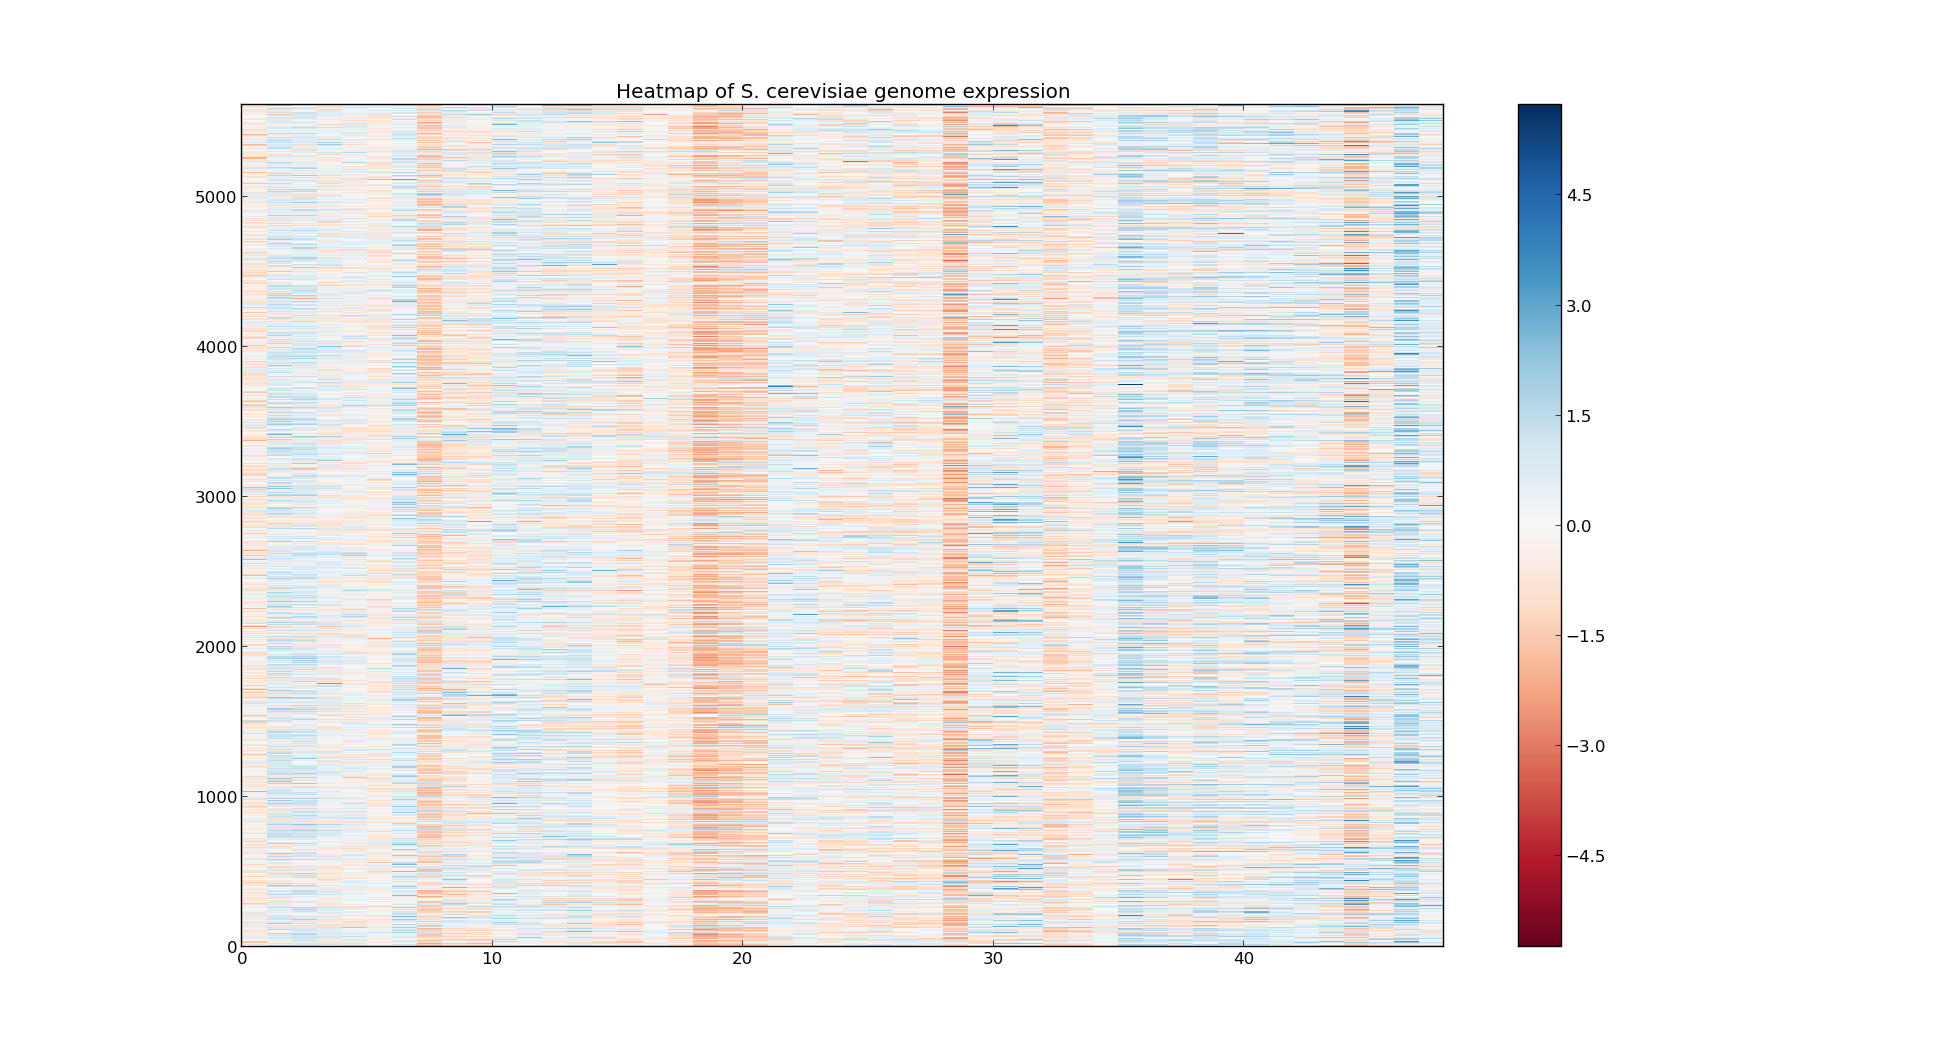
\includegraphics[width=1.4\linewidth]{02_heatmap_figure1_for_pnas.png}}
%\center{\hbox{\hspace{200pt}}\caption{A heatmap of the zscores of the genome expression time series data from Li and Klevecz(2006). Genome expression was normalized with respect to each gene in the genome of S. cerevisiae. Periodic patterns in the expression of almost every gene in the genome are apparent from the above figure.}\label{Figure1}}
%\end{figure}


%\begin{figure}[h]
%\centerline{ \hbox{\hspace{200pt}} 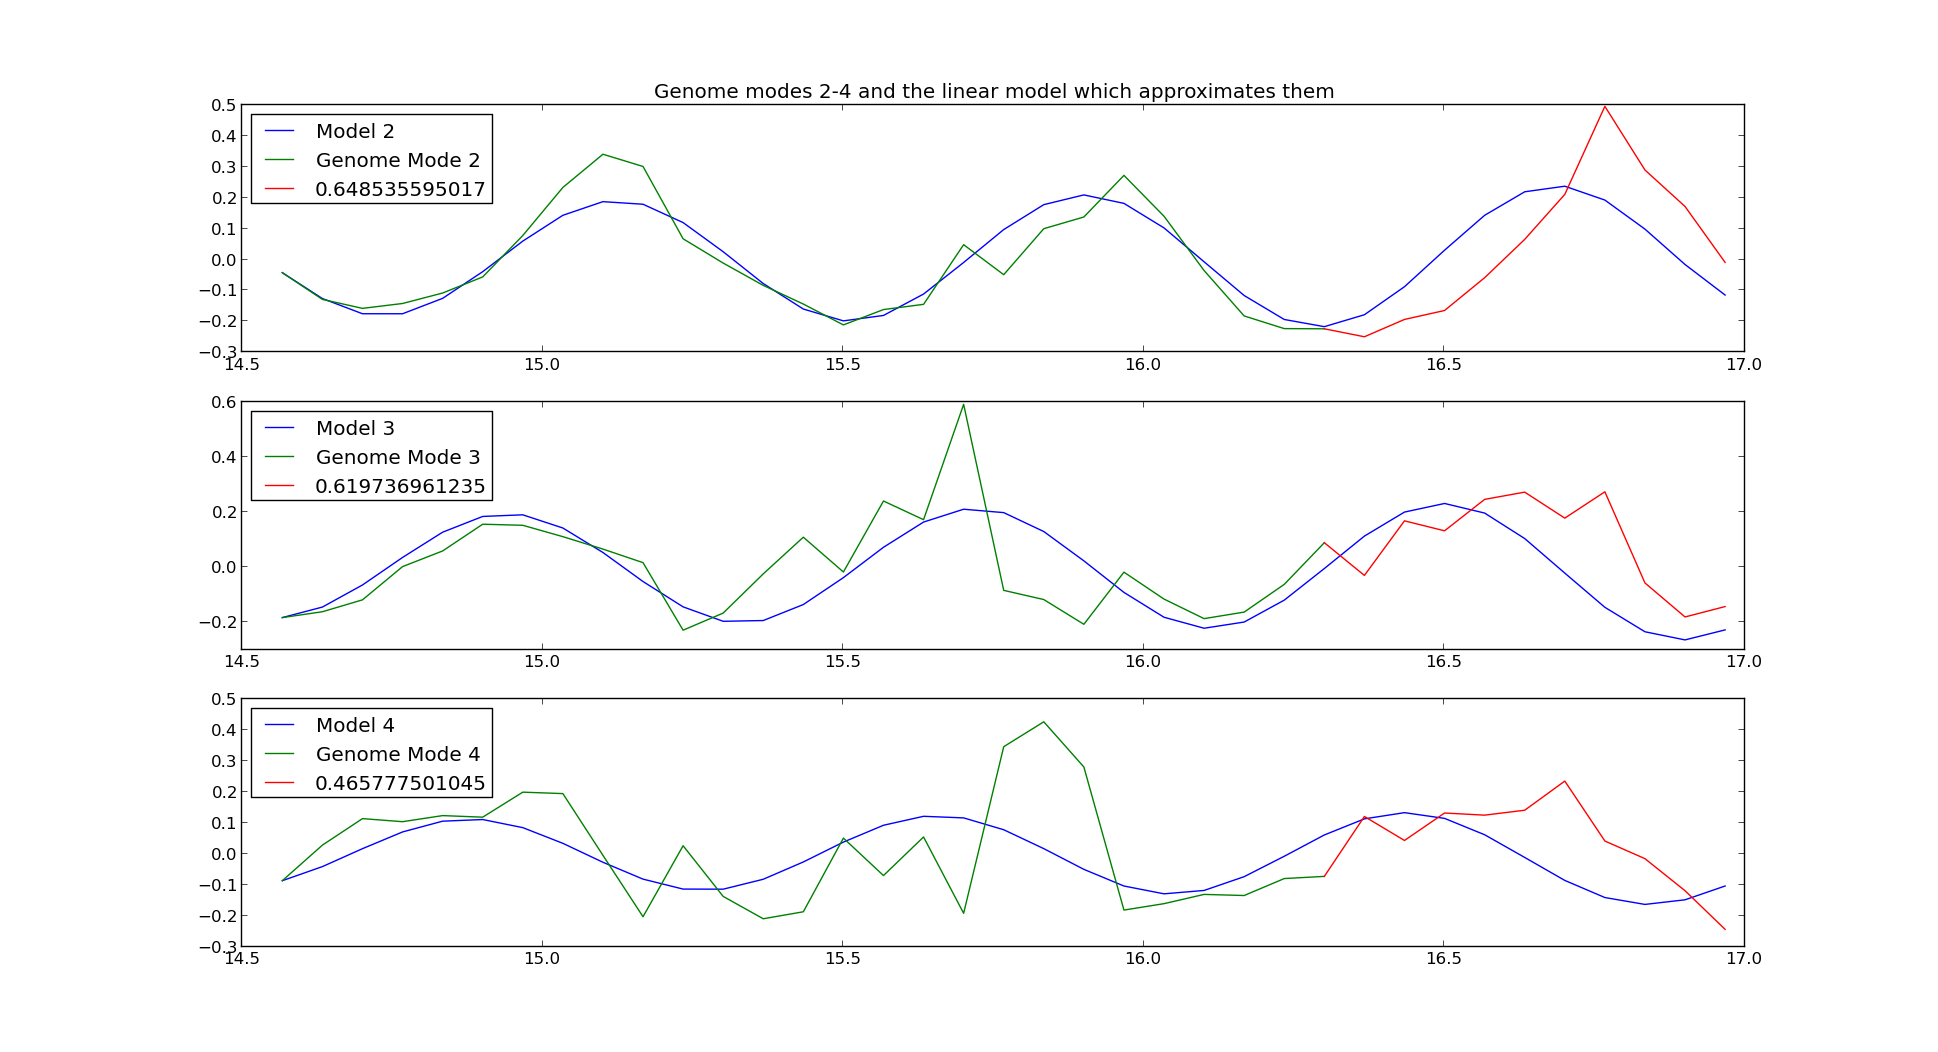
\includegraphics[width=1.4\linewidth]{03_figure2_for_pnas.png}}
%\center{\hbox{\hspace{200pt}}\caption{The second through fourth genome modes and the linear model which represents their dynamics are represented above in green and blue respectively. The test points in red are the result of projecting the second through fourth genome modes onto the last ten time points of the genome expression data from figure 1. The numerical values in the the legend are the Pearson Correlations between the model and the genome mode for the last ten time points. The overall correlation between the predictions of the model and the genome modes is 0.56334116.}\label{Figure2}}
%\end{figure}
%cumulativeVariance.png

\begin{figure}[h]
\centerline{ \hbox{\hspace{250pt}} 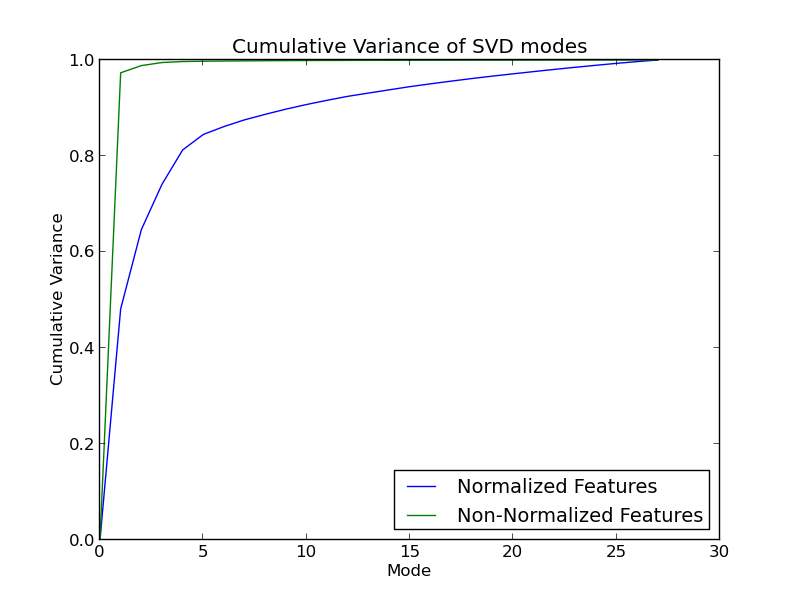
\includegraphics[width=0.8\linewidth]{cumulativeVariance.png}}
\center{\hbox{\hspace{200pt}}\caption{This is the caption}\label{Figure1}}
\end{figure}

\begin{figure}[h]
\centerline{ \hbox{\hspace{250pt}} 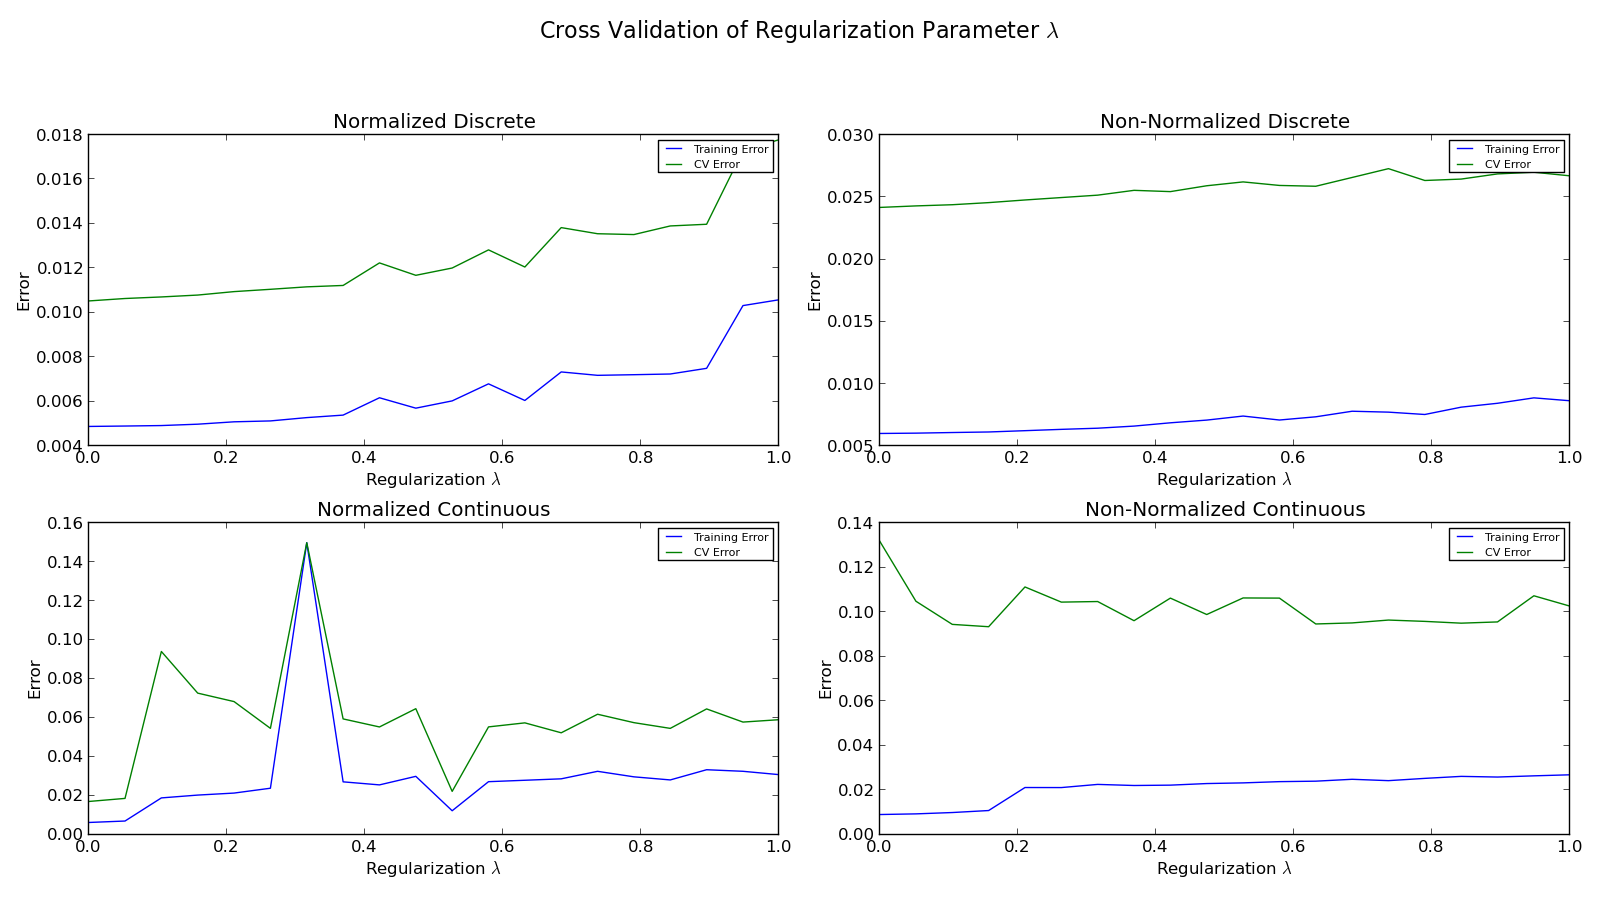
\includegraphics[width=1.0\linewidth]{crossValidationCurves.png}}
\center{\hbox{\hspace{200pt}}\caption{This is the caption}\label{Figure2}}
\end{figure}

\begin{figure}[h]
\centerline{ \hbox{\hspace{250pt}} 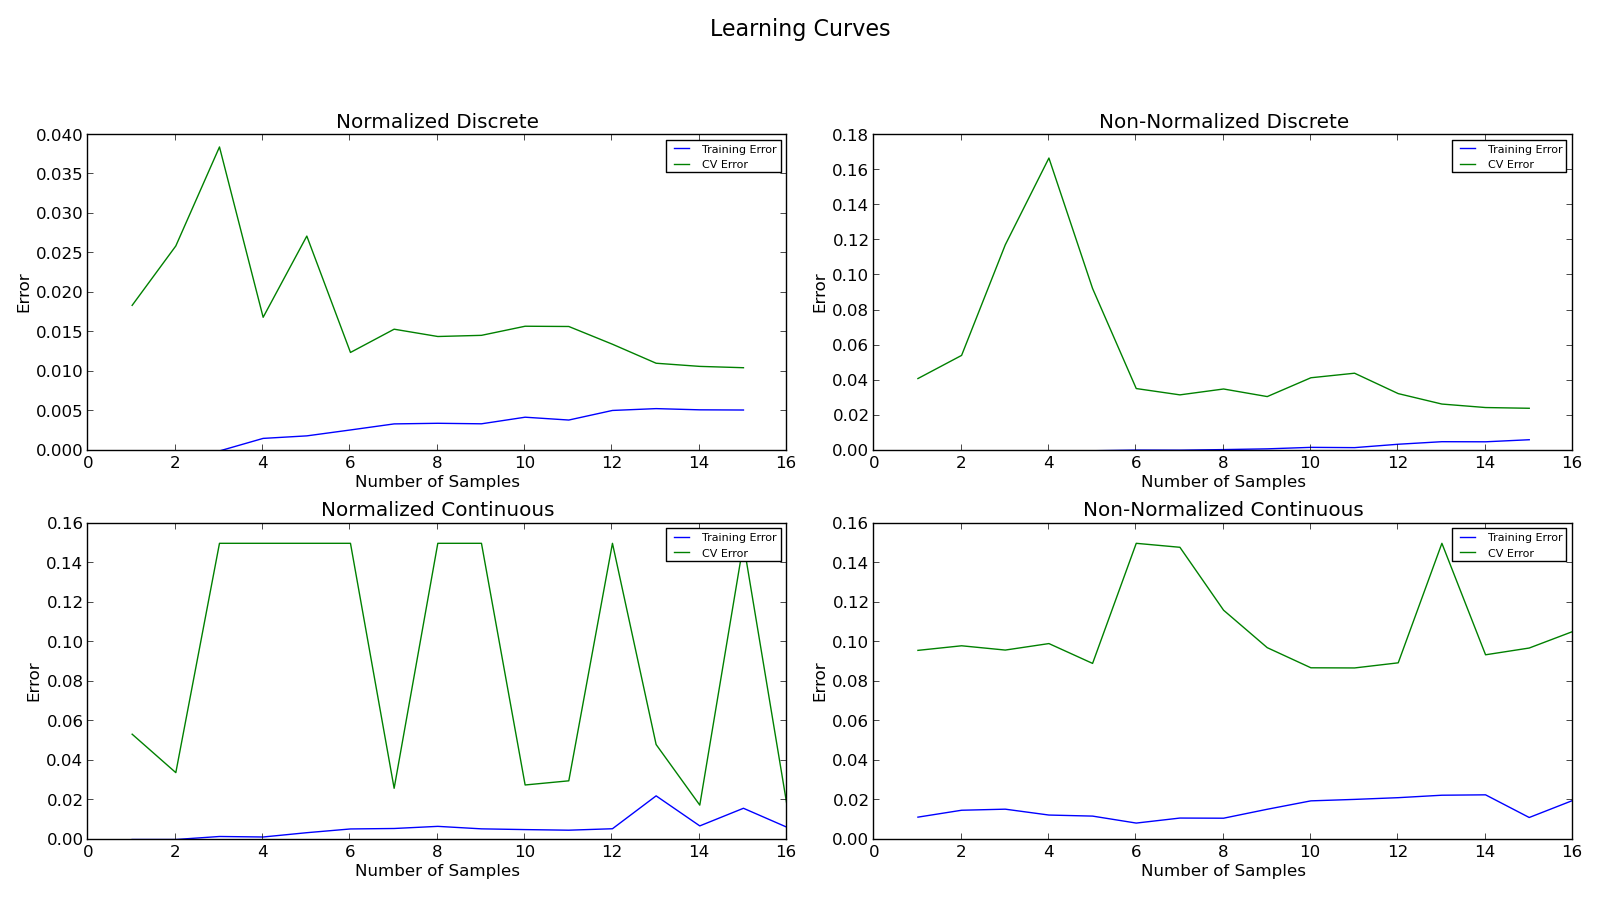
\includegraphics[width=1.0\linewidth]{learningCurves.png}}
\center{\hbox{\hspace{200pt}}\caption{This is the caption}\label{Figure3}}
\end{figure}

\begin{figure}[h]
\centerline{ \hbox{\hspace{250pt}} 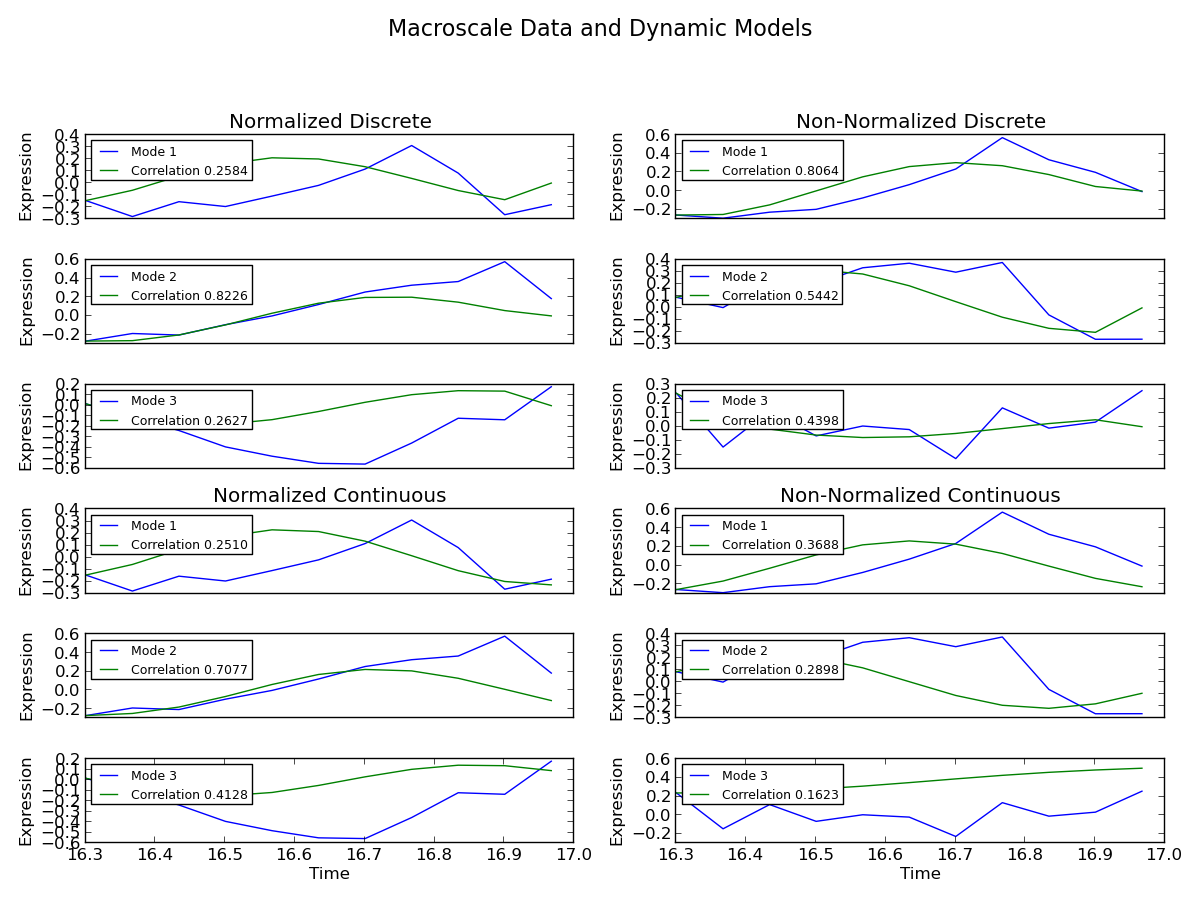
\includegraphics[width=1.0\linewidth]{macroscaleDynamics.png}}
\center{\hbox{\hspace{200pt}}\caption{This is the caption}\label{Figure4}}
\end{figure}


\begin{figure}[h]
\centerline{ \hbox{\hspace{250pt}} 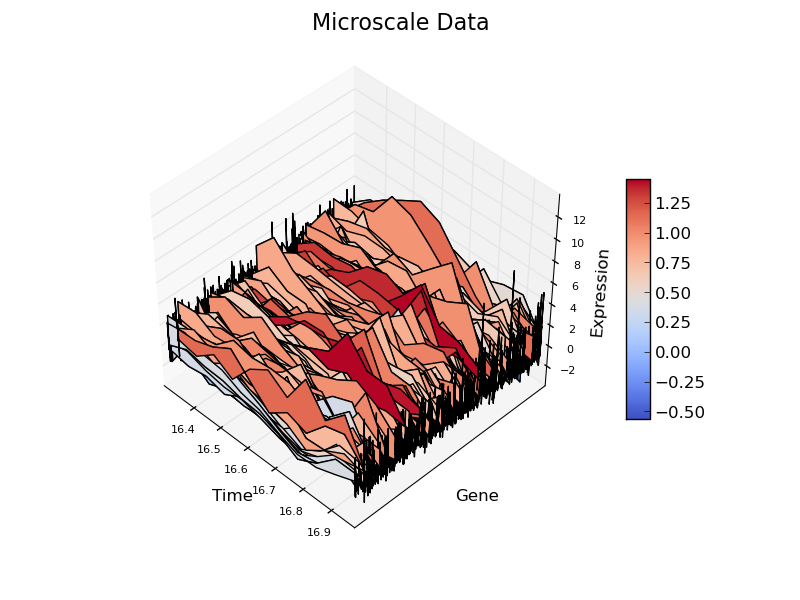
\includegraphics[width=1.1\linewidth]{microscaleTestSet.png}}
\center{\hbox{\hspace{200pt}}\caption{This is the caption}\label{Figure5}}
\end{figure}


\begin{figure}[h]
\centerline{ \hbox{\hspace{250pt}} 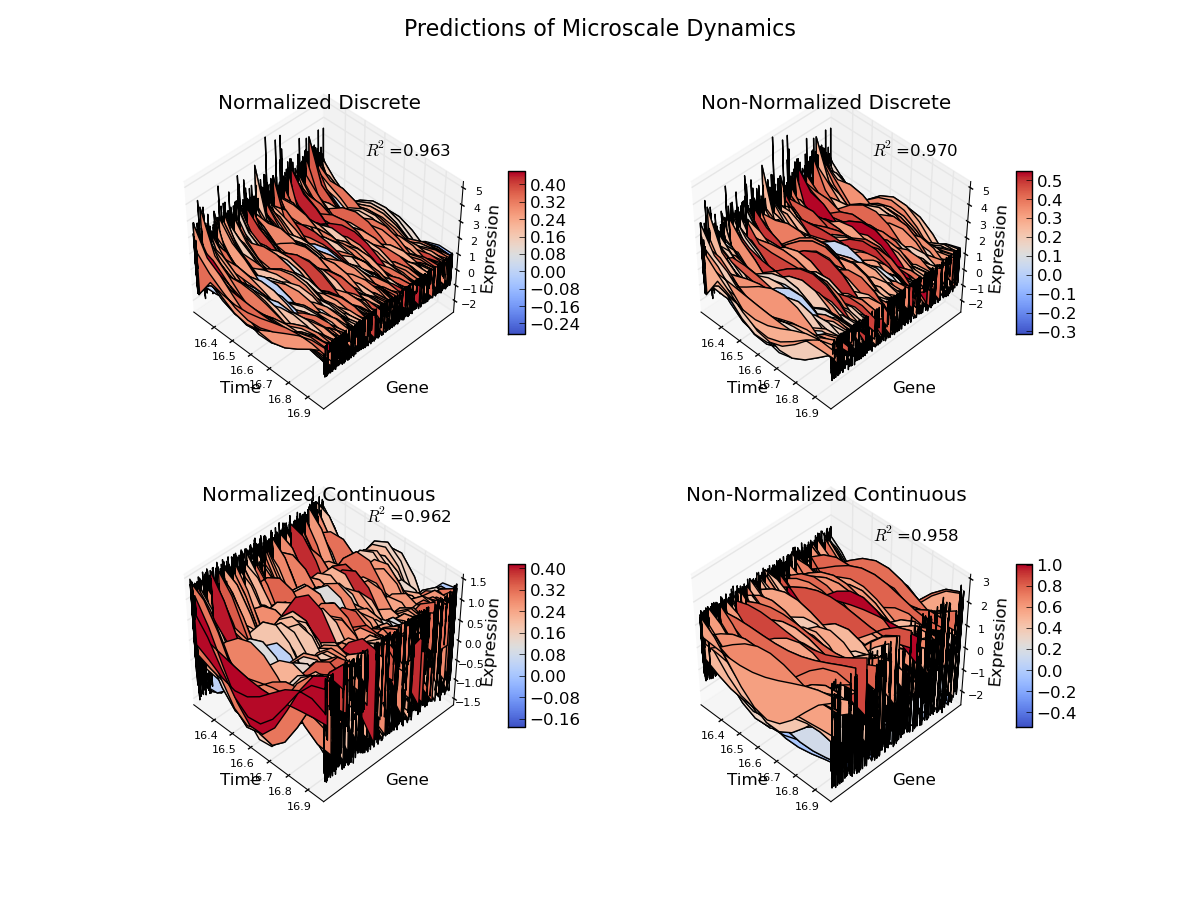
\includegraphics[width=1.1\linewidth]{microscaleDynamics.png}}
\center{\hbox{\hspace{200pt}}\caption{This is the caption}\label{Figure6}}
\end{figure}


\begin{figure}[h]
\centerline{ \hbox{\hspace{250pt}} 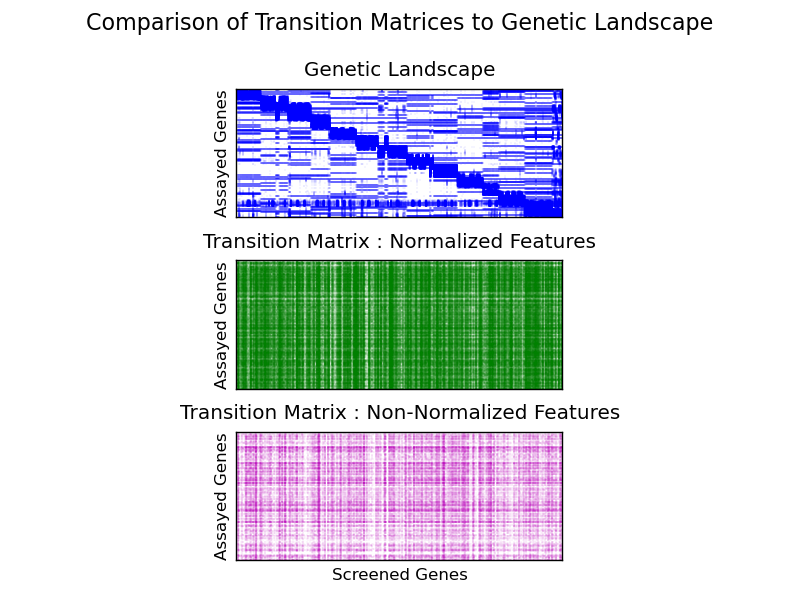
\includegraphics[width=1.1\linewidth]{comparisonAdjacency.png}}
\center{\hbox{\hspace{200pt}}\caption{This is the caption}\label{Figure7}}
\end{figure}

%% For Tables, put caption above table
%%
%% Table caption should start with a capital letter, continue with lower case
%% and not have a period at the end
%% Using @{\vrule height ?? depth ?? width0pt} in the tabular preamble will
%% keep that much space between every line in the table.

%% \begin{table}
%% \caption{Repeat length of longer allele by age of onset class}
%% \begin{tabular}{@{\vrule height 10.5pt depth4pt  width0pt}lrcccc}
%% table text
%% \end{tabular}
%% \end{table}

%%\begin{table}[h]
%\caption{Table caption}\label{sampletable}
%\begin{tabular}{l l l}
%\hline
%\textbf{Treatments} & \textbf{Response 1} & \textbf{Response 2}\\
%\hline
%Treatment 1 & 0.0003262 & 0.562 \\
%Treatment 2 & 0.0015681 & 0.910 \\
%Treatment 3 & 0.0009271 & 0.296 \\
%\hline
%\end{tabular}
%\end{table}

%% For two column figures and tables, use the following:

%% \begin{figure*}
%% \caption{Almost Sharp Front}\label{afoto}
%% \end{figure*}

%% \begin{table*}
%% \caption{Repeat length of longer allele by age of onset class}
%% \begin{tabular}{ccc}
%% table text
%% \end{tabular}
%% \end{table*}

%----------------------------------------------------------------------------------------

\end{document}
